\chapter{Code analysis of panoc}
The performance of the Matlab or Python code is not very relevant as it only generates source files, it's performance is not linked to the controller's performance. The generated C code on the other hand should have a good performance, as it determines the performance of the actual controller.

It is important to measure where most of the execution time is spent inside the algorithm. As this will indicate where to optimize the code. One way to measure this is by using profilers, in this chapter the results of the GNU profiler and the Intel profiler will be studied.

In order to get consistent results which profilers, the code execution must be long enough. And the problem that is being solved, must be sufficiently hard. So it will not converge in only a few steps. Because if it does converge in just a few steps, the cost function and its gradient will be the most dominant factor. They will take over 90\% of the execution time.The cost function and its gradient is generated by casadi and there's not much that can be done.

While if it does not converge in just a few steps, the quasi Newton method will be used. The buffer will be filled and the actual implementation of the algorithm will influence the performance significantly.

The problems used this chapter, will be the same as before in the chapter on simulations. The solution is displayed in figure~\ref{fig:solution nmpc problem analysis}. However as mentioned before the execution time must be sufficiently long. Solving just one optimal problem is not enough, even solving a whole simulation of problems is not enough. This is why 500 of these simulations will be executed sequentially while the profiler runs.

\begin{figure}[H]
	\centering
	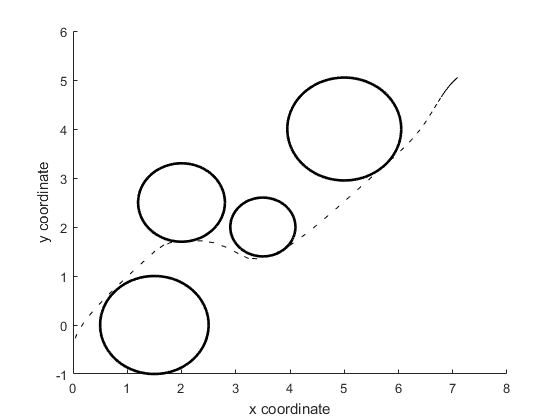
\includegraphics[width=0.5\textwidth]{intel_analysis/solution}
	\caption{solution nmpc problem analysis}
	\label{fig:solution nmpc problem analysis}
\end{figure}

\section{Intel Profiler}
The first profiler that will be discussed is Intel's Vtune Amplifier. In order to make the profiling easier, only one cost function will be used for both the cost function and its gradient. This means that evaluating the cost function, also means evaluating the gradient.

\subsection{Hot spot analysis}
The Intel profiler allows a hotspot analysis, which will find the functions that take most time when executing the simulations. The results are displayed in figure~\ref{fig:hotspot no mkl}.  It's quite clear from these results that the inner product and vector additions are two very dominance costs inside the algorithm.

The most dominant cost is the cost function and its gradient, as this function is generated by the casadi library. There's nothing that can be done about it's performance.

The inner product and vector additions can be implemented using Intel's MKL math library. These routines are fine-tuned BLAS routines and are one of the fastest on the market. Replacing inner products and vector additions with these routines however does not significantly change the performance of the algorithm.(results in firgure~\ref{fig:hotspot with mkl}) As the vectors used in this problem are too small to see a visible change. The BLAS functions just become the dominant cost now, it problem is not solved but moved.

It's true that the aim of the nmpc-codegen library is to provide control of the come use an embedded devices. And embedded devices will most likely not have BLAS routines, nevertheless this proves that putting a lot of time in optimizing the linear algebra routines might not always be very productive. The question is, how can the dependency on inner products and vector additions be reduced. The Intel profiler provides a function called bottom-up analysis. Bottom-up visualize, who is calling all these inner products and vector additions.

%The trailer model uses sines and cosines, these are also expensive operations. More on the sine and cosines later on.
\begin{figure}[H]
	\centering
	\begin{subfigure}[b]{0.45\textwidth}
		\centering
		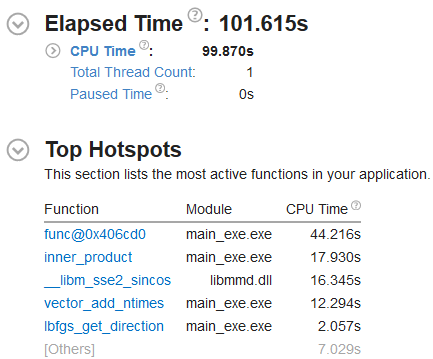
\includegraphics[width=1.2\textwidth]{intel_analysis/no_mkl}
		\caption{no mkl}
		\label{fig:hotspot no mkl}
	\end{subfigure}
	\hfill
	\begin{subfigure}[b]{0.45\textwidth}
		\centering
		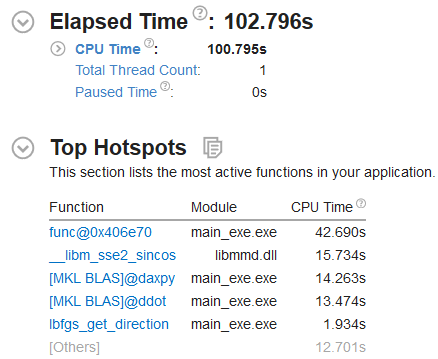
\includegraphics[width=1.2\textwidth]{intel_analysis/with_mkl}
		\caption{with mkl}
		\label{fig:hotspot with mkl}
	\end{subfigure}
	\caption{Hot spot analysis with Intel Vtune Amplifier 2018}
\end{figure}

Figure~\ref{fig:bottom-up analysis} provides a high-level view of the bottom-up analysis, figure~\ref{fig:detailed bottom-up analysis} provides a detailed view of the bottom-up analysis.From the detailed view it is clear that most of the inner product and vector addition function calls are coming from the L-BFGS algorithm. This underlines the importance of choosing the right buffer size for the quasi Newton method. To further illustrate this, figure~\ref{fig:Simulations with different buffer sizes} contains the simulation results for different buffer sizes.

\begin{figure}[H]
	\centering
	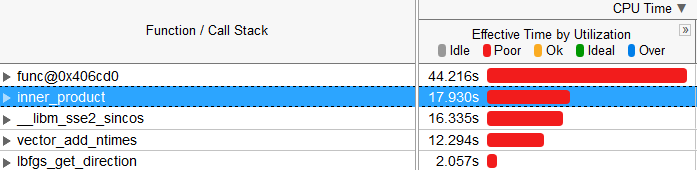
\includegraphics[width=0.7\textwidth]{intel_analysis/bottum_up}
	\caption{bottom-up analysis}
	\label{fig:bottom-up analysis}
\end{figure}

\begin{figure}[H]
	\centering
	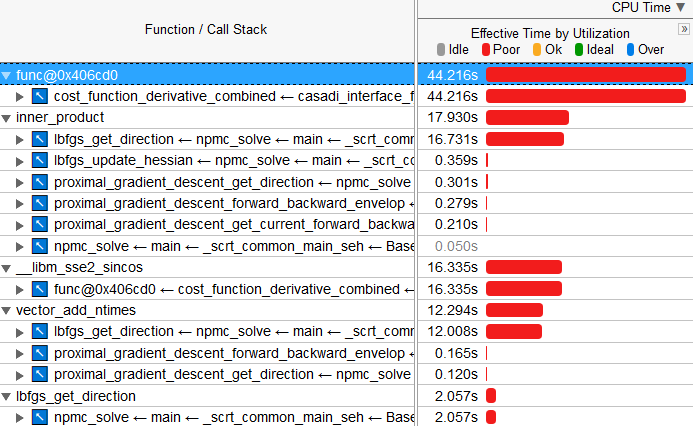
\includegraphics[width=0.7\textwidth]{intel_analysis/bottum_up_detailed}
	\caption{detailed bottom-up analysis}
	\label{fig:detailed bottom-up analysis}
\end{figure}

The number of iterations till convergence is illustrated in figure~\ref{fig:Simulations with different buffer sizes}, if you no L-BFGS is used then the algorithm clearly needs significantly more iterations. However if the L-BFGS method is used it will decrease the amount iterations till convergence. The bigger the size of the L-BFGS buffer the less iterations till convergence. However this does not mean that the algorithm will actually be faster, as a bigger buffer size means more inner products and vector additions. And as just illustrated with the profile, these inner products and vector additions are quite dominant in determining the execution time.

So it is imperative to not only take a large enough buffer, but also not take it too large as this will significantly impact the performance.

\begin{figure}[H]
	\centering
	\begin{subfigure}[b]{0.45\textwidth}
		\centering
		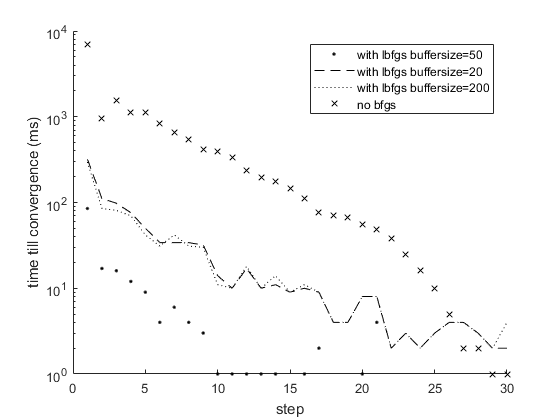
\includegraphics[width=1.2\textwidth]{compare_lbfgs_size/time_till_convergence}
		\caption{different lbfgs buffer time till convergence}
		\label{fig:different lbfgs buffer time till convergence}
	\end{subfigure}
	\hfill
	\begin{subfigure}[b]{0.45\textwidth}
		\centering
		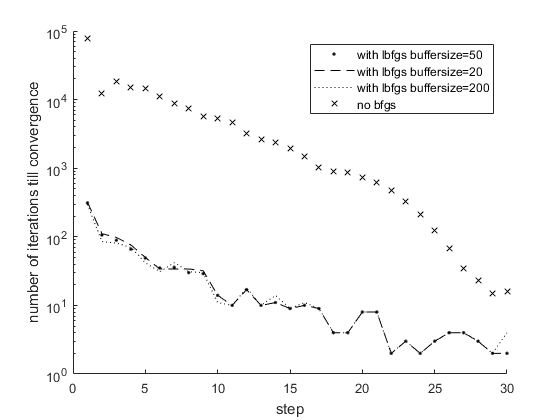
\includegraphics[width=1.2\textwidth]{compare_lbfgs_size/number_of_iterations}
		\caption{different lbfgs buffer iterations till convergence}
		\label{fig:different lbfgs buffer iterations till convergence}
	\end{subfigure}
	\caption{Simulations with different buffer sizes}
	\label{fig:Simulations with different buffer sizes}
\end{figure}

The opposite of a bottum-up  analysis is a top down analysis, which determines how  much time the  function spends inside the functions it calls. The results of this analysis is illustrated in figure~\ref{fig:no mkl top down}. Figure~\ref{fig:no mkl top down} indicates that about one third of the execution time is spend calculating the direction of the quasi Newton method. The two most dominant costs when calculating this are the inner products and the vector addition.

The rest of the time is mostly spent calculating the gradient and cost function. The proximal gradient method, is not so dependent upon inner products and vector additions. This is also visible in the caller callee analysis displayed in table~\ref{tbl:Caller Callee analysis}, about 61\% of the time is spent calculating the gradient. If the problem is easier to solve, or the buffer is smaller, then the cost of the gradient is even more dominant. And can easily go up to 80\% or 90\%. This is why a hard problem was used when profiling the algorithm. If an easy problem was used, then the results become irrelevant as the relative costs of the gradient will make everything else irrelevant.

\begin{figure}[H]
	\centering
	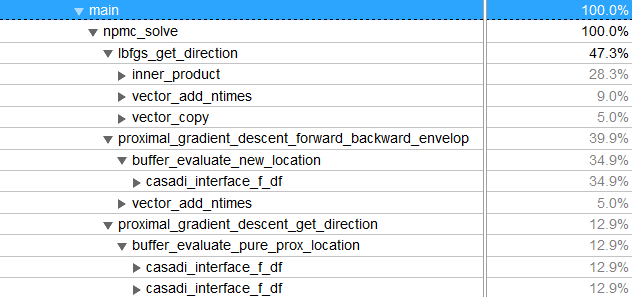
\includegraphics[width=0.7\textwidth]{intel_analysis/no_mkl_topdown}
	\caption{top down analysis}
	\label{fig:no mkl top down}
\end{figure}

\begin{center}
	\begin{tabular}{| l | c |}
		\hline
		Function&CPU Time: Total (\%) \\
		\hline
		casadi\_interface\_f\_df&61.2087\% \\
		proximal\_gradient\_descent\_forward\_backward\_envelop&36.9998\% \\
		buffer\_evaluate\_new\_location&34.7744\% \\
		lbfgs\_get\_direction&31.6374\% \\
		proximal\_gradient\_descent\_get\_direction&27.168\% \\
		buffer\_evaluate\_pure\_prox\_location&25.6641\% \\
		inner\_product&17.9297\% \\
		\_\_libm\_sse2\_sincos&16.335\% \\
		vector\_add\_ntimes&12.2935\% \\
		lbfgs\_update\_hessian&1.74661\% \\
		\hline
	\end{tabular}
	\captionof{table}{Caller/Callee analysis}
	\label{tbl:Caller Callee analysis}
\end{center}

\section{Valgrind callgrind}
The Intel profiler combined with the Visual Studio shell is incredibly easy to use and very productive. However it is a proprietary piece of software, and a rather expensive one. The Intel profiler uses the Intel compiler, which often times gives better results with numerical computations then using the GNU compiler. So it is worth while to investigate the results with the GNU compiler.

One way of profiling with the GNU compiler is using valgrind with the option callgrind as illustrated in listing~\ref{tbl:Caller Callee analysis}. Figure~\ref{fig:callgrid} displays the results of callgrind in a drawing. The relative execution time of the gradient is only 53\% instead of 61\% with the Intel compiler. It confirms the results obtained with the Intel profiler, as the inner products and vector additions are even more dominant here.

\begin{figure}[H]
	\centering
	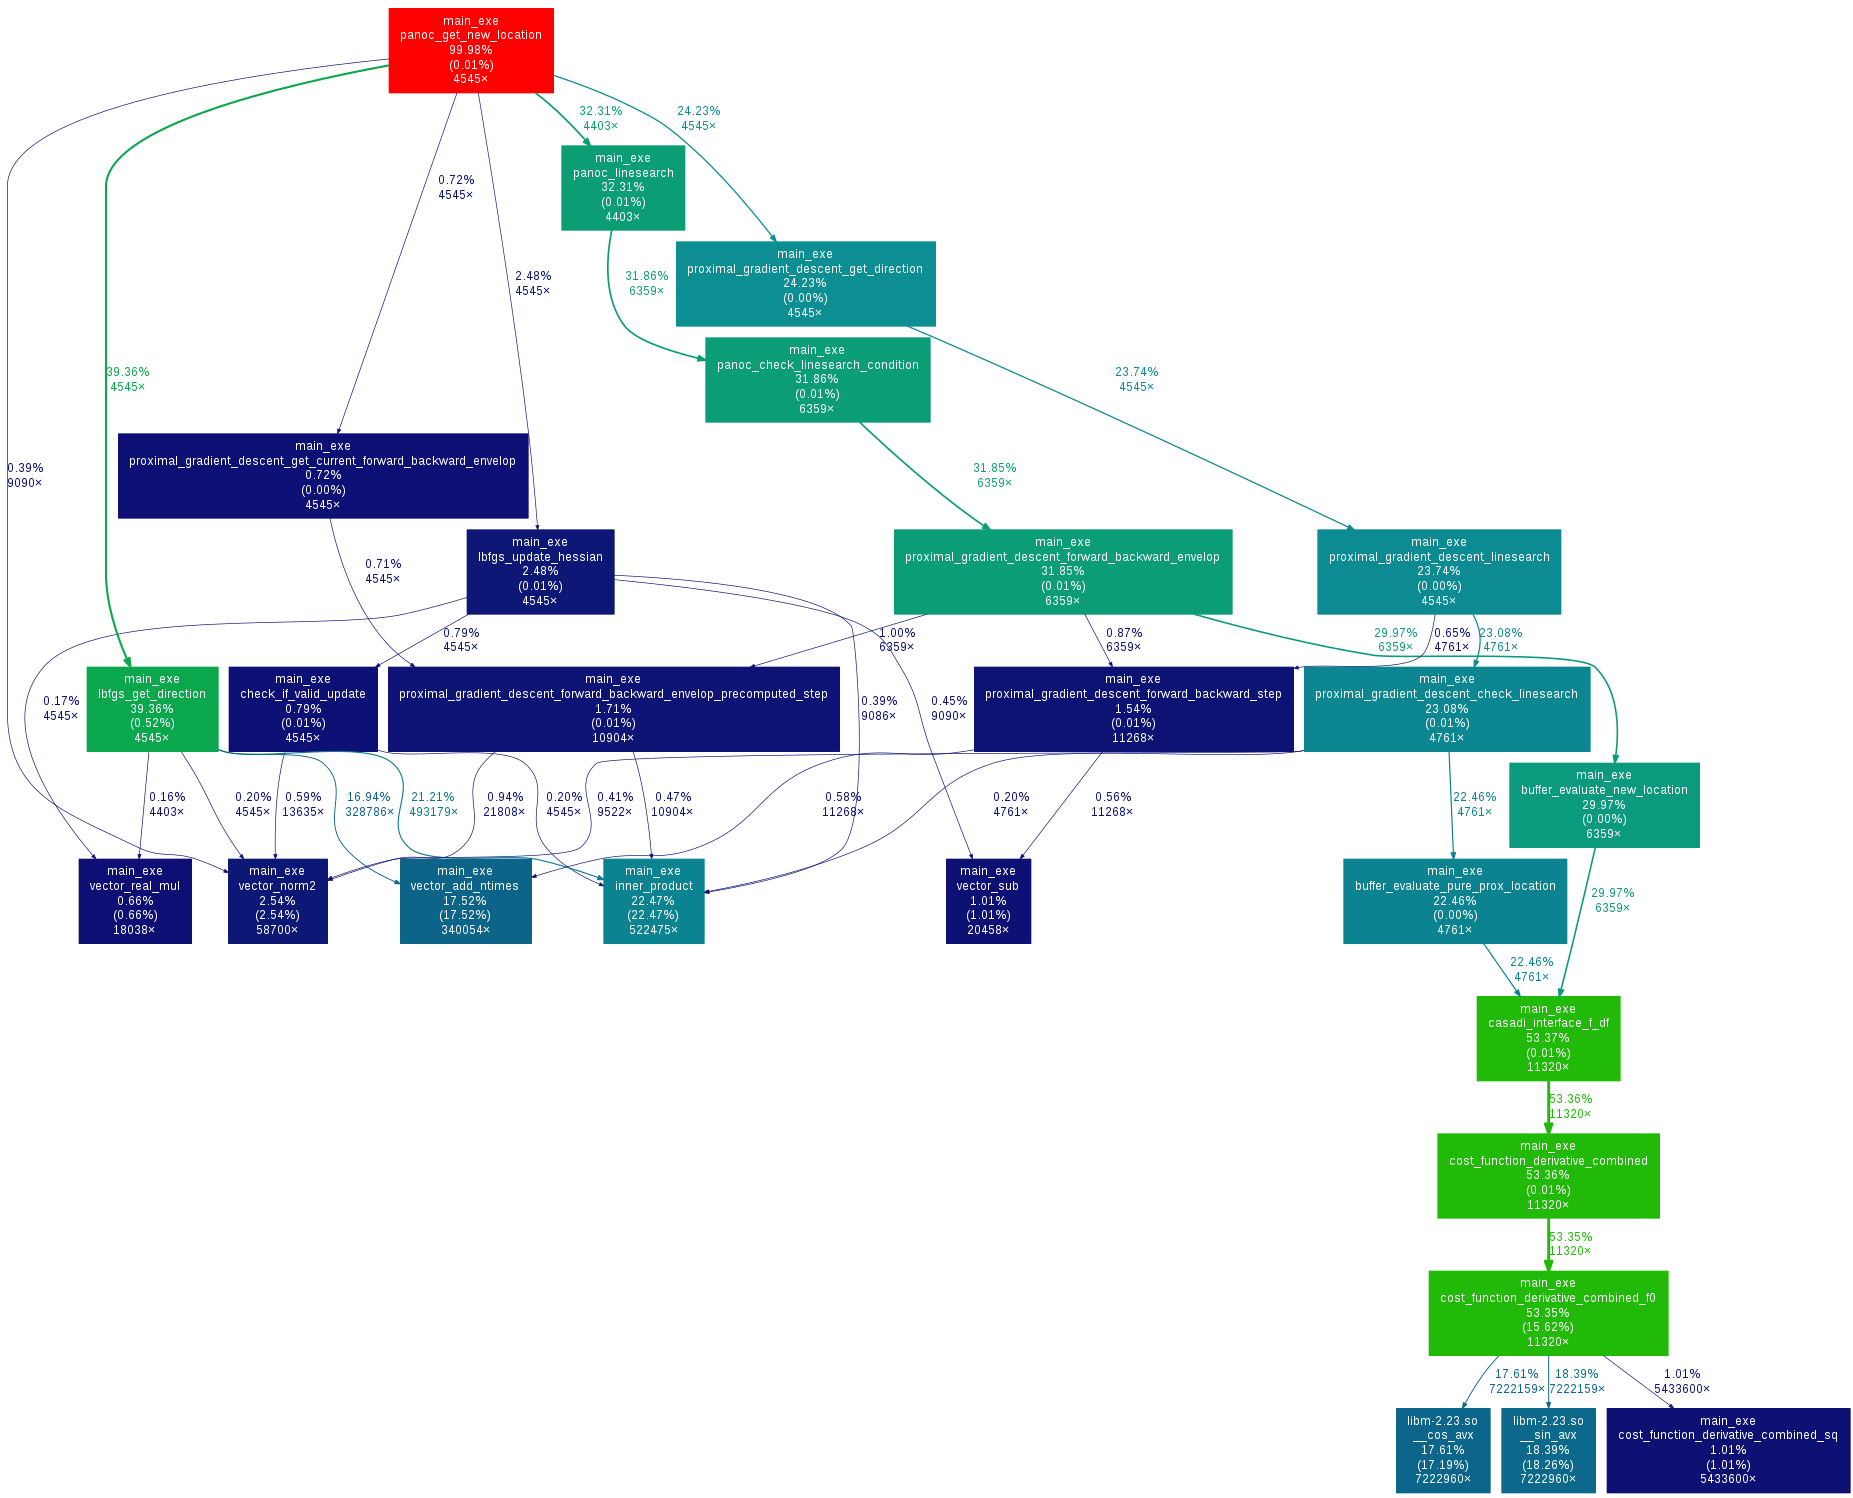
\includegraphics[width=1\textwidth]{callgrid/graph}
	\caption{callgrid}
	\label{fig:callgrid}
\end{figure}

\section{Conclusion}
The user should be careful when selecting the size of the buffer. If the buffer is too small the convergence will be slow. If the buffer is too large the quasi Newton method will require all lot more inner products and vector additions, which will significantly increase the time to convergence.
